\documentclass{article}
\usepackage{calc}
\usepackage{amsmath}
\usepackage{fancyhdr}
\usepackage{graphicx}
\usepackage{url}
\usepackage{tabularx}
\usepackage{xcolor,colortbl}
\usepackage{lastpage}
\usepackage{hyperref}
\usepackage{amsmath}
\usepackage{amssymb}
% format definitions 
\usepackage[most]{tcolorbox}
\usepackage[ddmmyyyy]{datetime}
\usepackage[a4paper, left=2cm,right=2cm,top=3.5cm,bottom=2.2cm, headsep=13pt, headheight=72pt]{geometry}
% macro definitions
\definecolor{Gray}{gray}{0.95}
\newcommand\titolo{ Sounding Canvas }
\newcommand\autore{ \href{https://luciamarock.wixsite.com/home}{Luciano Ciamarone \& Dora Motegh}}
\newcommand\versione{ \textbf{Ver.} 1.0 }
% header and footer definitions
\title{\titolo} 
\author{\autore} 
\lhead{ \titolo } 
\rhead{\autore}
\rfoot{Page \thepage \hspace{1pt} of \pageref{LastPage}}
\lfoot{\versione - \textbf{Date: }\date{\today}}
\cfoot{}
\pagestyle{fancy} 
\renewcommand{\footrulewidth}{0.4pt}
% links format definitions
\hypersetup{
	colorlinks=true,
	linkcolor=black,
	filecolor=black, % magenta  
	urlcolor=black,   % blue
}

\begin{document} 
\begin{titlepage}
\clearpage\maketitle
\thispagestyle{empty}
\end{titlepage}

\begin{centering}
	\section*{INDEX}
\end{centering}
\renewcommand*\contentsname{ }
\tableofcontents
\listoffigures
\listoftables
\bibliographystyle{unsrt}
\bibliography{References}

\newpage



\section{Introduction}
Sounding Canvas is an interactive audio-visual installation that transforms geometric paintings into responsive sound surfaces. Each artwork invites the viewer to become an active participant: by gently touching specific areas of the canvas, embedded capacitive sensors detect contact and trigger sonic responses in real time. A miniature computer mounted behind the canvas handles signal processing and sound generation, creating a seamless fusion of visual and auditory expression. \newline
The project was born from a collaboration between myself and my wife, who is a visual artist. While she designed the visual language of the canvases—merging elements of Persian calligraphy and musical notation—I developed the audio interaction layer and supporting technology. With backgrounds in both art and engineering, we combined our strengths to build artworks that go beyond observation, encouraging a tactile, performative engagement. \newline 
The motivation behind Sounding Canvas stems from a desire to dissolve the boundary between viewer and artwork. Instead of passive contemplation, we propose an intimate interaction: one that is immediate, sensorial, and even emotional. 
 The sound responses are not arbitrary; they are shaped by the visual features of the painting itself. \newline
A Convolutional Neural Network analyzes the artwork’s image and extracts parameters that inform the musical design, essentially creating a machine-assisted score. The audio engine, powered by custom algorithms and guided by a mathematical model, evolves dynamically based on user interaction history.
\newline
Ultimately, Sounding Canvas is a reflection on presence, gesture, and listening. It invites audiences to "listen with their hands"—to explore the tactile dimension of sound and the sonic potential of visual form. It is a meeting point between technology and emotion, structure and spontaneity, art and instrument.

\section{Artistic Concept}
 The visual component of the SoundingCanvas is the result of a semiographic investigation that blends elements of Persian calligraphy with Western musical notation. This hybrid script is not merely decorative—it is a symbolic expression of a personal and cultural journey. Dora, the visual artist behind the paintings (and also my wife), was born in Iran and later moved to Italy, where she encountered Western music, language, and culture (and me). The artwork thus becomes a metaphor for her life experience: the confluence of two distinct systems of meaning—visual, linguistic, and sonic—into a new, unified expressive form. \newline
 The paintings are not simple juxtapositions of visual, tactile, and sonic elements. Instead, they propose a deeper fusion—a newly invented language that lives at the intersection of these modalities. Each stroke and gesture on the canvas carries a semiotic weight that is not just visual, but also physical and acoustic. The canvas is a semiographic representation of this multi-sensory grammar: a new syntax born from the merging (not the layering) of sight, touch, and sound. This fusion gives rise to a new semantics, one that can only be experienced through interaction, and which cannot be reduced to any of its individual components.
\subsection{Background}
Dora graduated with a thesis titled: \emph{"A Study on the Use of Color in Film Scenography: Its Meaning and Effects on Visual Perception"} while mine was, instead \emph{"Research And Exploration Of Some Of The Factors That Most Influence People In Their Idea Of Musicality And In Their Approach To Listening"}, both of us were deeply interested in the impact that visual and auditory stimulation have on human perception and psychology. \newline 
Very soon (after we met) we started to work together on a FeedBack Ballet \cite{ballet} where an interactive stage set element would impact the very same music on which the performer danced. See also this paper \cite{accrocco_paper}. \newline 
Following our joint work on interactive audio scenographies for dance performances, our research interests naturally evolved toward questions of structure, perception, and cultural musical systems. During this period, I conducted an investigation into the automatic recognition of Dastgah—the modal system of Persian music—using statistical models such as Markov chains \cite{dastgah_markov}. This work focused on extracting meaningful features from audio signals and mapping them to perceptually relevant musical categories. The research helped me appreciate how mathematical models can be used not only to classify but also to reveal latent dimensions of music that are culturally and semantically rich. \newline
This focus on latent features and semantic meaning resonated deeply with Dora’s concurrent research into the symbolic use of color in cinematic scenography. These lines of inquiry—mine rooted in signal processing and statistical modeling, hers in visual semiotics and perception—came together in the conceptual foundation of the SoundingCanvas. The goal shifted from detection or classification toward creating a language, where visual forms, tactile interaction, and sound are not layered but fused into a new, expressive semiotic system.
\subsection{Birth of the Sounding Canvas project}
The decisive moment for the birth of the SoundingCanvas project came in November 2024, during a trip to Lanzarote in the Canary Islands. Surrounded by the island’s surreal landscapes, we made a firm commitment to bring our vision to life. By then, the core idea had already matured—both conceptually and technically. We knew how to realize it: we had the know-how, the artistic language, and the technology. The first prototype was based on an existing canvas that had previously been used in conjunction with the Accrocco, a scenographic stage element we had already employed in earlier works such as the Feedback Ballet. In many ways, we were assembling familiar ingredients: capacitive sensors, a custom audio engine, and machine learning models. We only needed to purchase the missing electronic components and adapt the existing setup. The canvas frame was already in place; it just required some restructuring to accommodate larger loudspeakers and embed the new interactive system. That marked the beginning of the first true SoundingCanvas.
\begin{figure}[h]
	\centering
	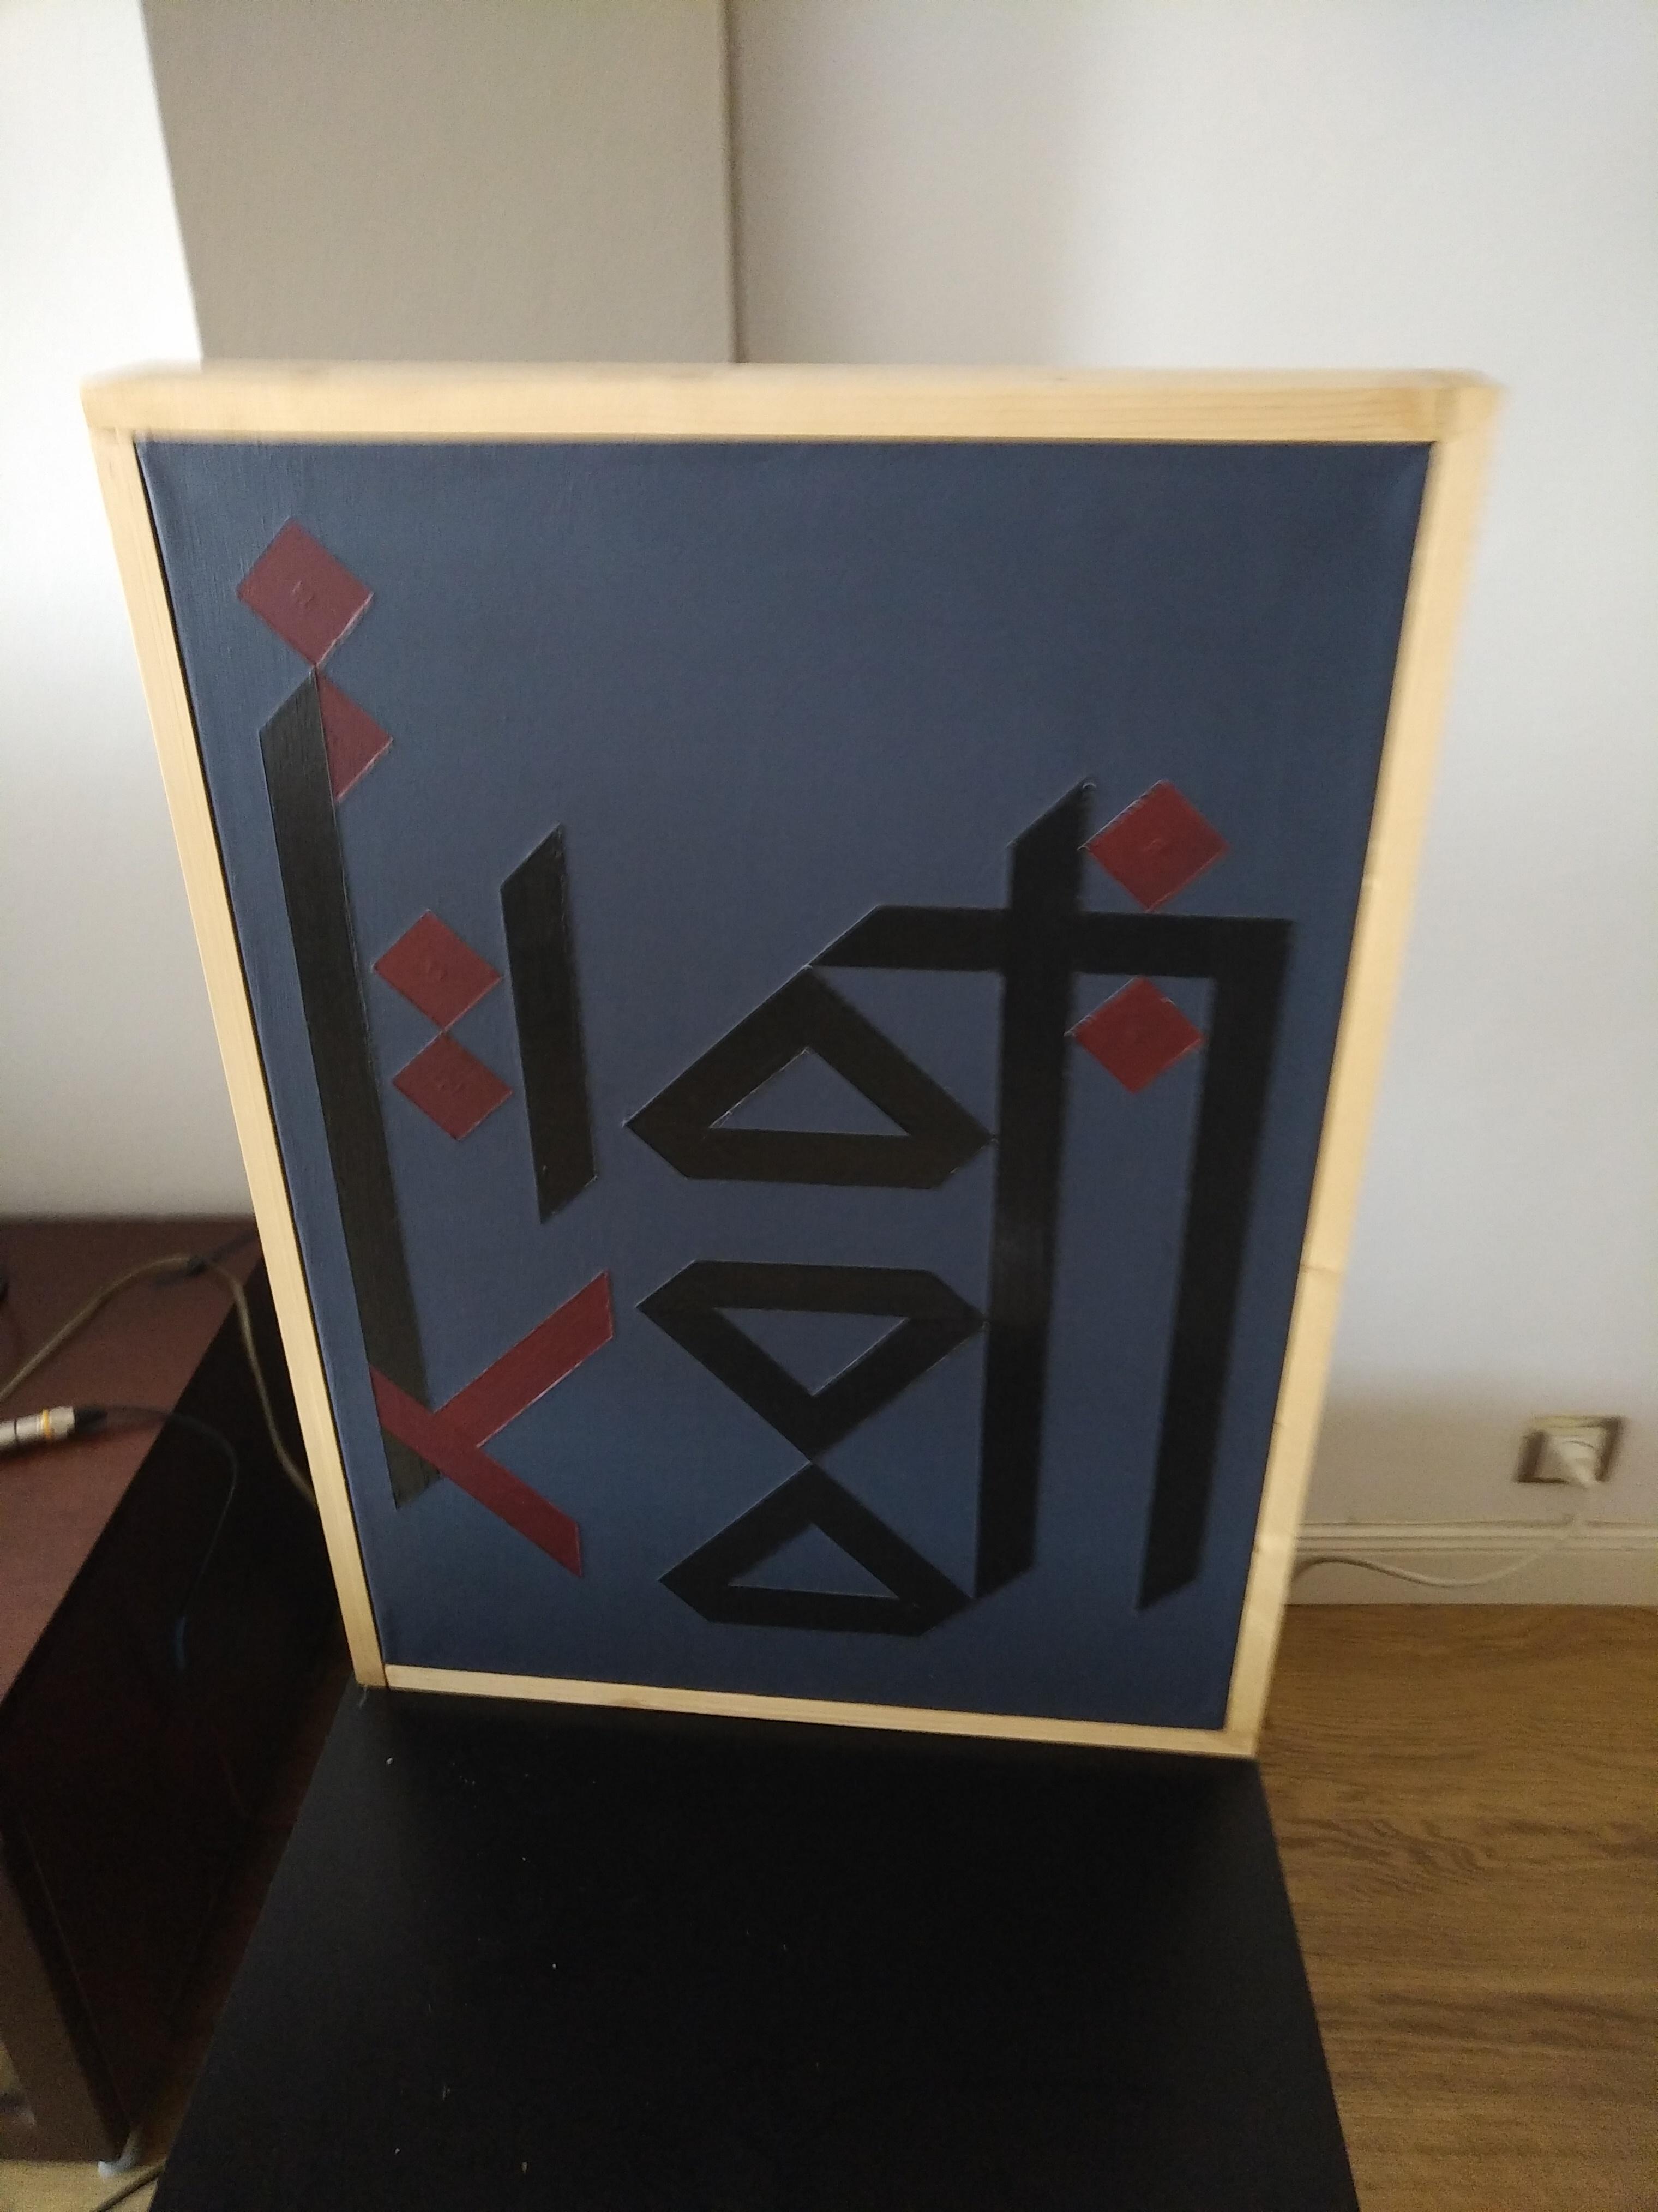
\includegraphics[height=10cm]{./images/script}
	\caption{Initial version of \emph{"Script of the Unsaid"}}
	\label{fig:script_of_the_unsaid}
\end{figure}

\section{Development}
In this section we provide a technical description of the project, we will refer to several concepts and most likely we will use the acronyms listed in Tab.~\ref{table:Acronyms}.
\begin{table}[h]
	\centering
	\begin{tabularx}{\textwidth} { 
			| >{\centering\arraybackslash}X
			| >{\centering\arraybackslash}X | }
		\hline
		\rowcolor{Gray}
		\textbf{Acronym} & \textbf{Description}\\
		\hline
		DSP & Digital Signal Processing \\
		\hline
		CNN & Convolutional Neural Network \\
		\hline
		AI & Artificial Intelligence \\
		\hline
		HW & Hardware \\
		\hline
		SW & Software \\
		\hline
		Pi & Raspberry Pi \\
		\hline
	\end{tabularx}
	\caption{Acronyms relevant to the SoundingCanvas project}
	\label{table:Acronyms}
\end{table}
The development of the Sounding Canvas project represents the convergence of diverse technical and artistic disciplines. Drawing from our backgrounds in scenography, psychoacoustics, and digital signal processing, we transformed a conceptual idea into a working interactive artwork. This section outlines the practical steps taken to design, prototype, and refine the system—from initial hardware integration to software architecture and machine learning components. Special attention is given to the challenges encountered during the creative process and the solutions that emerged through iterative experimentation.

\subsection{Hardware Design}
\subsubsection{Sensing}
The sensing mechanism of the Sounding Canvas is based on capacitive touch detection, implemented using an Arduino microcontroller and the \texttt{CapacitiveSensor} library. Each sensor is composed of a simple conductive element (typically aluminum foil) placed behind or integrated into the painted canvas surface. These sensors are connected to the Arduino using a resistor-capacitor configuration that allows the system to detect variations in capacitance when a human hand approaches or touches the canvas. \newline
The \texttt{CapacitiveSensor} library operates by measuring the time required for a pin to change logic state as it charges through a known resistor. This duration is directly influenced by the capacitance formed between the sensing electrode and the approaching body (e.g., a finger). The library essentially estimates this capacitance using the product of resistance and capacitance, referred to as the RC time constant:

\[
\tau = R \cdot C
\]
\noindent
where \( \tau \) is the time constant (i.e., delay), \( R \) is the resistor value in ohms, and \( C \) is the capacitance in farads. The delay measured across successive sampling cycles increases with higher capacitance, which allows us to infer touch proximity and intensity. \newline 
To improve stability and noise immunity, each sensor input is averaged over several iterations, and a threshold is dynamically adjusted based on environmental conditions. This simple yet effective solution enabled us to implement a multi-point touch interface that responds reliably to user interaction without requiring complex hardware or shielding, even in the relatively uncontrolled environments of public exhibitions.
\footnote{\href{https://luciamarock.github.io/Projects/technicalities/tech\_report.html}{Some more in depth technicalities can be found here}}
\begin{figure}[h]
	\centering
	\includegraphics[height=6.2cm]{./images/sensors}
	\caption{Connection of the Sensors behind the canvas}
	\label{fig:sensors}
\end{figure}

\subsubsection{Computing}
The main computing unit of the Sounding Canvas is a Raspberry Pi 4 Model B, selected for its balance between computational power, compactness, and low power consumption. This board is equipped with a 1.5\,GHz quad-core ARM Cortex-A72 CPU and is responsible for real-time audio playback, touch event processing, and communication with peripheral devices. \newline 
Touch data is acquired via an Arduino Uno, which handles the capacitive sensors and transmits processed readings to the Raspberry Pi through a serial USB connection. The communication protocol between the two devices is kept intentionally simple: the Arduino sends a stream of numeric values (e.g., one per sensor), delimited and parsed by the Raspberry Pi in a Python script that listens on the appropriate serial port. \newline 
The choice to offload the capacitive sensing logic to the Arduino allows for more efficient use of system resources. The Raspberry Pi is thereby dedicated to more demanding tasks such as:

\begin{itemize}
	\item managing audio sample selection and triggering,
	\item running digital signal processing routines,
	\item hosting the machine learning modules for sound mapping,
	\item controlling speaker outputs through a HiFiBerry Amp2 HAT.
\end{itemize}
\noindent
This distributed architecture ensures modularity, robustness, and flexibility. The system can be extended easily by adding more sensors or reprogramming the Arduino with minimal changes to the Raspberry Pi's software stack.

\subsubsection{Amplifying}
The Sounding Canvas uses a HiFiBerry Amp2 HAT (Hardware Attached on Top) as its dedicated audio amplifier. This add-on board is directly mounted onto the Raspberry Pi 4 Model B via the GPIO header, enabling seamless integration and minimal cabling. The Amp2 features a high-quality Class-D amplifier capable of delivering up to 30\,W per channel into 4\,$\Omega$ speakers, providing enough headroom for small to medium-sized installation spaces. \newline 
Notably, the HiFiBerry Amp2 is the only component in the system that receives external power. It is powered by a robust DC power supply unit—specifically, an Elektron PM510—which provides a regulated 13.8\,V output with up to 10\,A continuous current and 12\,A peak capacity. When connected, the Amp2 not only powers itself but also powers the Raspberry Pi through its onboard voltage regulator, simplifying the system’s power topology. \newline
Two full-range passive loudspeakers are connected directly to the screw terminals of the Amp2 board. The speaker outputs are stereo (left and right channels), and the cables are routed internally through the frame of the canvas to ensure a clean aesthetic and minimize electromagnetic interference. \newline 
This amplification setup offers a compact, reliable, and high-fidelity audio solution that is ideal for an interactive sound installation, ensuring the sonic output is both spatially immersive and acoustically articulate.

\subsubsection{Assembling}
The final step in the hardware development was the physical assembly of the system components into a unified, reliable structure. At the core of this phase was the use of a medium-density fibreboard (MDF) panel, which played a dual role: it provided structural support and created a barrier between the sensitive front-facing sensor area and the electronic and audio components mounted on the rear. See Fig.~\ref{fig:assembled}. \newline 
This MDF panel was custom-cut to match the dimensions of the canvas and fixed to its rear frame. On this panel, we securely mounted all the main hardware components, including the Raspberry Pi with its HiFiBerry Amp2 HAT, the Arduino microcontroller, and the power distribution elements. This separation was essential not only for mechanical stability but also to isolate the touch-sensitive area from electromagnetic and mechanical disturbances generated by the electronics. \newline 
The two passive loudspeakers were also mounted directly onto the MDF panel in a symmetric arrangement, allowing optimal sound diffusion while preserving the aesthetic and acoustic coherence of the artwork. Power and audio signal cabling were neatly routed and fixed along predefined channels, minimizing movement and interference, and ensuring long-term durability during transportation and exhibition. \newline 
The sensing layer, made of conductive elements like aluminum foil connected via 1\,M$\Omega$ resistors, was affixed to the front side of the canvas, while sensor wires were carefully passed through the MDF to reach the Arduino inputs. This internal routing further preserved the visual purity of the canvas while enabling responsive and stable sensor readings.

\begin{figure}[h]
	\centering
	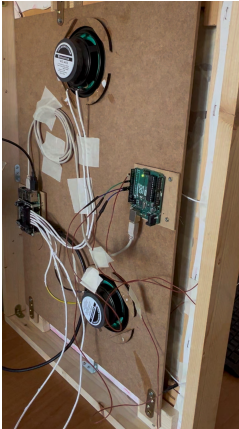
\includegraphics[height=10cm]{./images/assembled}
	\caption{Rear view of the Sounding Canvas \emph{"Script of the Unsaid"}}
	\label{fig:assembled}
\end{figure}
\noindent
The assembling phase concluded with thorough testing of physical connections and system stability, marking the transition from a set of prototype components to a self-contained, gallery-ready interactive artwork.

\subsection{Software Architecture}
The software architecture of the Sounding Canvas project is designed to seamlessly integrate sensor input, audio processing, system management, and artificial intelligence components into a cohesive and responsive interactive artwork. It consists of modular layers that communicate efficiently to deliver real-time sound synthesis triggered by user touch on the canvas. \newline 
At its core, the system captures capacitive sensor data via an Arduino microcontroller, which is responsible for low-level event detection and communication with the main processing unit. The Raspberry Pi hosts the audio engine that processes incoming events, generates spatialized sound output, and manages system operations such as startup and safety monitoring. \newline 
In parallel, an AI component is integrated to enhance the system’s expressive capabilities, enabling more sophisticated audio-visual mappings and machine learning-driven adaptations. \newline 
This section breaks down the software into four main components, each responsible for specific functionalities:
\begin{itemize}
	\item \textbf{Arduino Interface \& Event Manager}: Handles sensor data acquisition and event messaging.
	\item \textbf{Audio Engine}: Manages real-time sound synthesis, processing, and output.
	\item \textbf{Startup \& System Services}: Ensures automated operation, graceful shutdowns, and system safety.
	\item \textbf{AI Component}: Implements machine learning models for intelligent sound and interaction.
\end{itemize}
\noindent
Together, these components provide a robust, flexible, and maintainable framework supporting the interactive experience of the Sounding Canvas.

\subsubsection{Arduino Interface \& Event Manager}
The Arduino Interface plays a crucial role in bridging the physical sensing hardware with the higher-level software logic running on the Raspberry Pi. It is responsible for collecting raw capacitive touch data from the sensor electrodes mounted behind the canvas and transmitting meaningful interaction events to the main system. \newline 
The Arduino aggregates CapacitiveSensor data and periodically transmits it over a USB serial connection to the Raspberry Pi. A custom Python module on the Raspberry Pi acts as a listener and parser for this serial data stream. The module maintains a queue of recent readings and applies event detection logic to identify new touch events, sustained contact, or release events. \newline 
To ensure responsiveness and avoid false triggers, the system employs a hysteresis mechanism and configurable thresholds. For example, a touch is only registered if the measured signal exceeds a given activation threshold for a sustained number of readings. This approach reduces noise and ensures reliable operation even in environments with fluctuating electromagnetic conditions. \newline 
Once events are detected, they are forwarded to the \textit{Event Manager}, a central coordination module responsible for triggering corresponding actions within the system. These actions include activating sound playback through the Audio Engine, updating visual feedback, or logging interaction data. \newline 
Beyond simple event forwarding, the Event Manager also performs adaptive learning based on user interaction patterns. Until now, the system has used adaptive Markov models to infer probabilities of sequential gestures and transitions over time. This probabilistic model allows the system to react in a more context-aware manner, anticipating likely next events and tailoring the sonic or visual response accordingly. \newline 
Current development includes the exploration of Recurrent Neural Networks (RNNs) as a more powerful approach for modeling and detecting complex, temporally extended interaction sequences. This opens up the possibility for deeper temporal understanding of user behavior, enriching the perceptual and expressive potential of the artwork. \newline 
The modular design of the Arduino Interface and Event Manager ensures a clear separation between the low-level hardware communication and the high-level behavioral logic. This structure makes the system maintainable and extensible — new sensor types or behaviors can be added with minimal impact on the overall architecture.

\subsubsection{Audio Engine}
The Audio Engine is responsible for generating and playing the auditory output in response to user interaction events. In its current implementation, it primarily uses pre-recorded sound samples that are mapped to different types of interactions, as interpreted by the Event Manager. These sound samples are triggered with minimal latency, allowing for a responsive and intuitive audio-visual experience. \newline 
Each interaction event—such as a touch, a release, or a complex gesture—is associated with one or more audio responses. These mappings can be fixed or dynamically modulated depending on the temporal context, as inferred by the probabilistic models or learning algorithms in the Event Manager. This creates a tight coupling between gesture and sound, where patterns of user behavior can influence both the selection and variation of sonic output. \newline 
Beyond playback of fixed audio samples, the system is evolving towards real-time sound synthesis, offering significantly greater flexibility and expressive potential. Unlike sample playback, synthesis enables dynamic control over low-level parameters of sound such as frequency, amplitude, envelope, timbre, and spatialization. These parameters can be continuously modulated in response to user actions, environmental conditions, or internal system states. \newline 
To guide this real-time synthesis, we apply formal constraints inspired by the domain of Physics. In particular, we are currently exploring mathematical models derived from Loop Quantum Gravity and other advanced physical theories as a basis for shaping and modulating the sonic structures. These models provide a rich space of parameters and relations that can be mapped onto audio synthesis algorithms. For example, discrete geometric structures or evolution rules from these theories can be interpreted as governing principles for waveshape formation, modulation, or spectral behavior. \newline 
This approach leads to a synthesis engine that is not only responsive but also semantically meaningful—creating sounds that embody formal, structured complexity rather than arbitrary noise or repetition. The resulting sonic output often mirrors the layered and emergent quality of the visual artwork, reinforcing the perceptual metaphor that the system is built upon. 

\subsubsection{Startup \& System Services}
To ensure autonomous operation and smooth installation of the Sounding Canvas, we implemented a robust startup and shutdown management system based on \texttt{systemd} and scheduled jobs.

\paragraph{Automatic Startup}
At boot, a \texttt{systemd} service is configured to launch the main application automatically. This includes initializing serial communication with the Arduino board and starting the touch-to-sound software running on the Raspberry Pi. The \texttt{.service} file also manages dependencies and logging, allowing the system to recover gracefully after a power cycle or reboot.

\paragraph{Scheduled Shutdown}
To optimize power consumption and prevent unnecessary wear, the system includes a scheduled shutdown mechanism using a \texttt{cron} job. This can be configured to power down the Raspberry Pi at a fixed time each day, or after a certain period of inactivity.

\paragraph{Thermal Protection}
A lightweight Python script periodically checks the Raspberry Pi’s CPU temperature. If the temperature exceeds a predefined safety threshold (typically around 80–85\textdegree C), the system initiates a clean shutdown to prevent hardware damage. This self-protection mechanism is particularly useful in enclosed installations or in galleries with fluctuating environmental conditions.

\paragraph{Integration with Power Management}
The shutdown procedure is complemented by the use of smart plugs or relay-controlled power outlets, which can cut off power completely a few minutes after the Raspberry Pi has shut down. This ensures that the entire system—including amplification—is powered off safely without user intervention.

\paragraph{Installation Advantages}
This combination of automated startup, temperature monitoring, and clean shutdown makes the Sounding Canvas installation plug-and-play. Gallery staff or curators are not required to interact with the electronics: powering the artwork is reduced to switching the smart plug on or off. This design simplifies deployment and ensures long-term stability in exhibition environments.

\subsubsection{AI Component}
The AI component of the Sounding Canvas project plays a central role in linking the visual and auditory domains through abstract, learned representations. Rather than relying on conventional classification or prediction, we employ Convolutional Neural Networks (CNNs) in an unconventional way: the classification head is discarded, and only the convolutional body is retained to extract high-level features from the canvas image. This results in a multidimensional feature space representing the visual semantics of the artwork. \newline 
Similarly, a multidimensional representation of the audio domain is constructed using a hybrid combination of signal analysis techniques, including spectral descriptors (e.g., MFCCs, spectral centroid), temporal features, and energy dynamics. These features, once normalized and embedded, form a parallel space that encodes the auditory characteristics of the sound output. \newline 
Conceptually, we interpret both the image feature space $\mathcal{V}$ and the audio feature space $\mathcal{A}$ as vector spaces with their own bases. That is, we assume the existence of bases $\{v_i\}$ for $\mathcal{V}$ and $\{a_j\}$ for $\mathcal{A}$ such that any visual or auditory percept can be represented as a linear combination of these basis vectors.

\paragraph{Mathematical Formalization}

Let $\mathbf{x} \in \mathbb{R}^n$ be a feature vector extracted from the CNN representation of the canvas (visual domain), and let $\mathbf{y} \in \mathbb{R}^m$ be the corresponding vector in the audio space. \newline 
We define two basis matrices:
\[
V = [v_1 \, v_2 \, \ldots \, v_n] \in \mathbb{R}^{n \times n}, \quad A = [a_1 \, a_2 \, \ldots \, a_m] \in \mathbb{R}^{m \times m}
\]
Assuming a linear transformation exists between these two spaces, we can express the transformation as:
\[
\mathbf{y} = T \mathbf{x}, \quad \text{with} \quad T \in \mathbb{R}^{m \times n}
\]
\noindent
Here, $T$ is the transformation matrix that "translates" between the visual and auditory perspectives. This matrix is learned or estimated using a mapping technique such as canonical correlation analysis (CCA), regression, or a neural network trained on paired visual-audio examples.

\paragraph{Conceptual Implication}

This mathematical transformation is not merely a computational trick—it serves as a metaphor for the artwork itself. The Sounding Canvas embodies a new semantics, a fusion of perception through image, touch, and sound. The mapping from one space to another becomes a symbolic act: a change of basis that redefines meaning, turning sensory input into a new interpretative language. \newline
In this sense, the transformation $\mathbf{y} = T \mathbf{x}$ mirrors the artistic goal: to offer a perceptual and cognitive shift, unveiling hidden correlations and resonances between visual composition and sonic experience.

\subsection{Multi-Canvas Networking}
A defining feature of the \textit{Sounding Canvas} project is its capacity to function not only as a standalone interactive artwork but as part of a distributed network of canvases. Each canvas, while physically independent and potentially separated by vast geographic distances, remains virtually connected through a centralized server. This interconnection enables novel forms of artistic dialogue, real-time data exchange, and synchronized sonic responses between installations. \newline 
The communication architecture follows a server-centric model. Every canvas establishes a persistent WebSocket connection with a central server deployed on the internet. This server acts as a message broker, coordinating and relaying interaction data between canvases. For example, a touch interaction on one canvas can be captured locally, encoded, and transmitted to the server, which then routes this data to one or more remote canvases. These remote units, upon receiving the signal, can generate corresponding sonic or visual responses, thus establishing a sense of telepresence and remote co-authorship. \newline
Each canvas is identified by a unique \texttt{client\_id}, allowing the server to maintain a registry of active canvases. The server supports bi-directional communication, enabling both broadcasting and targeted messaging between nodes. This allows for diverse interaction models: from one-to-many synchronization (e.g., triggering a shared harmonic gesture across all canvases), to one-to-one private interactions (e.g., initiating a musical motif in response to a specific remote canvas). \newline
Beyond the technical framework, the impact of this networked approach is fundamentally human. By turning abstract touch into sound, and transmitting that sound across distance, the system fosters a form of emotional presence. Imagine a mother in one country gently interacting with her canvas and triggering a soundscape in her child's room thousands of kilometers away. Without words or screens, a subtle gesture becomes a shared, intimate experience—transcending physical separation and evoking presence through art.


\section{Licensing and Ownership}
\textit{Sounding Canvas} © 2024 by Luciano Ciamarone and Dora Motegh is licensed under the \href{https://creativecommons.org/licenses/by-nc-sa/4.0/}{Creative Commons Attribution-NonCommercial-ShareAlike 4.0 International License}.
\newline
This license allows others to remix, adapt, and build upon the work non-commercially, provided they give appropriate credit to the original creator and license their new creations under the same terms. Commercial use is not permitted without explicit permission.
\newline
For source code and related resources, please visit the GitHub repository at \href{https://github.com/luciamarock/SoundingCanvas}{github.com/luciamarock/SoundingCanvas}.  
To learn more about the author and the broader context of this work, visit \href{https://luciamarock.github.io/}{luciamarock.github.io}. \newline 
This work has been entirely conceived, implemented, and authored by Luciano Ciamarone and Dora Motegh. \newline 
All conceptual and technical contributions presented herein are original unless explicitly referenced.


\section{Exhibitions \& Links}
Past installations and exhibitions (updated until the date of this document):
\begin{itemize}
	\item Ca l’Isidret, Barcelona (2025), from  April 8, to Jun 2
	\item MORPHOS – Temporary Identities 2025, Palazzo Albrizzi-Capello, Venice - April 24 to May 09
\end{itemize}
Links: 
\begin{itemize}
	\item \href{https://doramoteque-faf94c.webflow.io/}{Dora's Website}
	\item \href{https://www.youtube.com/@doradynamicdesign}{Youtube Channel}
	\item \href{https://www.instagram.com/doramoteque/}{Dora's IG}
	\item \href{https://luciamarock.github.io/news/soundingcanvas.html}{SoundingCanvas news page}
\end{itemize}

\newpage
\begin{thebibliography}{References}
	\bibitem{ballet}
	Luciano Ciamarone \& Dora Motegh. 
	\textit{Feedback Ballet}.  
	Available at: \url{https://luciamarock.github.io/Projects/technicalities/feedback_ballet.html}  	
	
	\bibitem{accrocco_paper} 
	Ciamarone, Motegh, Di Donato,
	\textit{An Interactive Audio Scenography for Dance Performance}.  
	Independent Research, Rome; Academy of Fine Arts, Frosinone; Goldsmiths, University of London.  
	\texttt{luciano.ciamarone@libero.it}, \texttt{negar.motegh@gmail.com}, \texttt{b.didonato@gold.ac.uk}.
	
	\bibitem{dastgah_markov}
	Luciano Ciamarone, Baris Bozkurt, and Xavier Serra. 
	\textit{Automatic Dastgah Recognition using Markov Models}. 
	In: \textit{Perception, Representations, Image, Sound, Music}. 
	CMMR 2019, Marseille. Published by Springer, ISBN: 978-3-030-70210-6.
	
\end{thebibliography}
\end{document}